% !TEX root = main.tex
% !TEX spellcheck = it-IT
\documentclass[12pt,a4paper,twoside,openright,titlepage]{book}	
	
\usepackage[binding=5mm]{layaureo}
\usepackage[swapnames]{frontespizio}
\usepackage[english,italian]{babel}
\usepackage{microtype}
\usepackage{hyperref}
\usepackage{tabularx}
\usepackage{listings}
\usepackage{float}
\usepackage{changepage,calc}
\usepackage{emptypage}
\usepackage{indentfirst}
\usepackage{fancyhdr}
\usepackage{relsize}
\usepackage{bookmark}
\usepackage{lipsum}	
\usepackage[footnote,smaller]{acronym}
\usepackage{pdfpages}
\setlength{\headheight}{15pt}
\usepackage{graphicx}

\graphicspath{ {images/} }

\usepackage[autostyle,italian=guillemets]{csquotes}
\usepackage[style=philosophy-modern,hyperref,backref,natbib,backend=biber,defernumbers=true]{biblatex}
\addbibresource{Bibliografia.bib}

%\title{Library Box}
%\date{2020-12-10}
%\author{Andrea Calici (10490117)}

\begin{document}
%% !TEX root = Tesi.tex
% !TEX spellcheck = it-IT
\newcommand{\myName}{Andrea Calici}
\newcommand{\myMatricola}{944717}
\newcommand{\myTitle}{Titolo della Tesi}
\newcommand{\myUni}{Politecnico di Milano}
\newcommand{\myFaculty}{Scuola di Ingegneria Industriale e dell'Informazione}
\newcommand{\myDegree}{Computer Science and Engineering}
\newcommand{\myThesis}{Tesi di Laurea Magistrale}
\newcommand{\myDepartment}{Dipartimento di Informatica}
\newcommand{\myProf}{Prof.~Luciano~Baresi}
\newcommand{\myLocation}{Milano}
\newcommand{\myTime}{Aprile 2014}
\newcommand{\myAcademicYear}{2020--2021}
\newcommand{\myUrlUni}{www.polimi.it}
\newcommand{\myUrlFaculty}{www.ingindinf.polimi.it}

\newenvironment{sistema}%
	{\left\lbrace\begin{array}{@{}l@{}}}%
	{\end{array}\right.}
%
% epsilon theta rho phi
\renewcommand{\epsilon}{\varepsilon}
\renewcommand{\theta}{\vartheta}
%\renewcommand{\rho}{\varrho}
\renewcommand{\phi}{\varphi}
%
\renewcommand{\vec}{\mathbf} 	% vettori in tondo nero
%

% Impostazioni degli acronimi
\makeatletter
\def\bflabel#1{{\textbf{\textsf{#1}}\hfill}}
\renewenvironment{AC@deflist}[1]%
{\ifAC@nolist%
\else%
\begin{list}{}%
{\settowidth{\labelwidth}{\textbf{\textsf{#1}}}%
\setlength{\leftmargin}{\labelwidth}%
\addtolength{\leftmargin}{\labelsep}%
\renewcommand{\makelabel}{\bflabel}}%
\fi}%
{\ifAC@nolist%
\else%
\end{list}%
\fi}%
\makeatother

\hyphenation{OpenFOAM}
\hyphenation{Matlab}
\hyphenation{bash}


\includepdf{fronte/fronte.pdf}
%\pdfbookmark[1]{Frontespizio}{Frontespizio}
\begin{frontespizio}

\Preambolo{\renewcommand{\frontsmallfont}[1]{\small Matr.}}
\Margini{1.5cm}{1.5cm}{1.5cm}{1.5cm}
\Istituzione{Politecnico di Milano}
\Logo[2.5cm]{images/logo}
\Divisione{Scuola di Ingegneria Industriale e dell'Informazione}
%\Dipartimento{Meccanica}
\Corso{Computer Science and Engineering}
\Titoletto{Tesi di Laurea Magistrale}
\Titolo{Progetto Salvavita}
\Candidato[944717]{Andrea Calici}
\Relatore{Prof.~Luciano~Baresi}
\Annoaccademico{2020--2021}
\Punteggiatura{}
\Rientro{1cm}
\end{frontespizio}
\pagenumbering{gobble}
%\maketitle
% !TEX root = ../Tesi.tex
% !TEX spellcheck = it-IT
%\tableofcontents
\cleardoublepage
%
% ------------------------------------------------------------------------ %
%
% Indice Generale
%
\pdfbookmark{\contentsname}{tableofcontents}
%
\setcounter{tocdepth}{2}
%
\tableofcontents
%
\cleardoublepage
%
% ------------------------------------------------------------------------ %
%
% Indice delle Figure
%
\phantomsection
%
\pdfbookmark{\listfigurename}{lof}
%
\listoffigures
%
\cleardoublepage
%
% ------------------------------------------------------------------------ %
%
% Indice delle Tabelle
%
\phantomsection
%
\pdfbookmark{\listtablename}{lot}
%
\listoftables
%
\cleardoublepage
%
% ------------------------------------------------------------------------ %
%
% Indice dei Listati di Programma
%
\phantomsection
%
\pdfbookmark{\lstlistlistingname}{lol}
%
\lstlistoflistings
%
\cleardoublepage
% !TEX root = ../Tesi.tex
% !TEX spellcheck = it-IT
\cleardoublepage
\phantomsection
\pdfbookmark{Ringraziamenti}{ringraziamenti}
\chapter*{Ringraziamenti}
\lipsum[1]

\medskip

Desidero inoltre ringraziare esplicitamente:
\begin{description}
\item[{\scshape Esplicito1}] per vari motivi;
\item[{\scshape Esplicito2}] per altri motivi;
\item[{\scshape Esplicito3}] per puro piacere, senza particolari motivi.
\end{description}

\bigskip
 
\noindent\textit{Milano, Mese 2021}
\hfill A.~C.
% !TEX root = ../Tesi.tex
% !TEX spellcheck = it-IT
\cleardoublepage

\phantomsection

\pdfbookmark{Sommario}{Sommario}

\begingroup

\let\cleardoublepage\relax
\let\cleardoublepage\relax

\chapter*{Sommario}

\lipsum[1]

\medskip

\noindent \textbf{Parole chiave:} 
PoliMi,
Tesi,
LaTeX,
Scribd

%\clearpage

\selectlanguage{english}

\pdfbookmark{Abstract}{Abstract}

\chapter*{Abstract}

Text of the abstract in english\dots\\
\lipsum[1]

\medskip

\noindent \textbf{Keywords:} 
PoliMi,
Master Thesis,
LaTeX,
Scribd

\selectlanguage{italian}
\endgroup			
%% !TEX root = ../Tesi.tex
% !TEX spellcheck = it-IT
% ------------------------------------------------------------------------ %
%
% ------------------------------------------------------------------------ %
% 	ACRONIMI
% ------------------------------------------------------------------------ %
%
\cleardoublepage
%
\chapter*{Acronimi}
%
\markboth{Acronimi}{Acronimi}	% headings
%
\begin{acronym}[MMG]	% tra [ ] inserire l'acronimo pi� lungo
%
% ------------------------------------------------------------------------ %
%
% tra [ ] inserire come deve apparire l'acronimo nel testo
%
% ------------------------------------------------------------------------ %
%
\begin{otherlanguage*}{english}
%
\acro{CFD}[CFD]{Computational Fluid Dynamics}

{\smaller Computational Fluid Dynamics is a branch of fluid mechanics that uses numerical methods and algorithms to solve and analyze problems that involve fluid flows. Computers are used to perform the calculations required to simulate the interaction of liquids and gases with surfaces defined by boundary conditions.\\
\href{http://en.wikipedia.org/wiki/Computational_fluid_dynamics}{www.en.wikipedia.org}
\par}
%
\end{otherlanguage*}
%
% ------------------------------------------------------------------------ %
%
\acro{HPC}[HPC]{High Performance Computing}

{\smaller In informatica con il termine High Performance Computing (calcolo ad elevate prestazioni) ci si riferisce alle tecnologie utilizzate da computer cluster (insieme di computer connessi tra loro tramite una rete telematica) per creare dei sistemi di elaborazione in grado di fornire delle prestazioni molto elevate, ricorrendo tipicamente al calcolo parallelo.\\
\href{http://it.wikipedia.org/wiki/High_Performance_Computing}{www.it.wikipedia.org}
\par}
%
% ------------------------------------------------------------------------ %
%
\begin{otherlanguage*}{english}
%
\acro{OpenFOAM}[OpenFOAM]{Open source Field Operation And Manipulation}

{\smaller The OpenFOAM\textregistered\ CFD Toolbox is a free, open source CFD software package which has a large user base across most areas of engineering and science, from both commercial and academic organisations. OpenFOAM has an extensive range of features to solve anything from complex fluid flows involving chemical reactions, turbulence and heat transfer, to solid dynamics and electromagnetics. It includes tools for meshing, notably \emph{snappyHexMesh}, a parallelised mesher for complex CAD geometries, and for pre- and post-processing. Almost everything (including meshing, and pre- and post-processing) runs in parallel as standard, enabling users to take full advantage of computer hardware at their disposal.\\
\href{http://www.openfoam.com/}{www.openfoam.com}
\par}
%
\end{otherlanguage*}
%
% ------------------------------------------------------------------------ ------------------------------------------------------------------------ %
%
\end{acronym}
%
% ------------------------------------------------------------------------ %

\addcontentsline{toc}{chapter}{Definizioni e Acronimi}
\chapter*{Definizioni e Acronimi}
\section*{Definizioni}
In questa sezione verrà presentata una lista di termini comuni e di utile comprensione che verranno utilizzati nel corso della trattazione:
\begin{itemize}
\item Utente: il generico utente finale dell'applicazione e comprensivo delle figure del cittadino e del volontario;
\item Cittadino: utente finale che è in grado di accedere ai propri dati sanitari e salvavita e generare attraverso l'applicazione documenti di utilità;
\item Volontario: utente finale dell'applicazione che rappresenta la figura di riferimento per l'inserimento dei dati di natura pratica del cittadino e che può avere accesso al sistema sia per la fase di inserimento di informazioni, sia per eseguire funzioni di utilizzo dei dati;
\item Carta d'Identità Salvavita: documento contenente il codice QR salvavita e i dati sanitari di emergenza del cittadino;
\item Fascicolo Sanitario Elettronico: strumento che permette di ricostruire la storia clinica del cittadino con la presenza dei dati e dei documenti sanitari dello stesso;
\item Scheda Sanitaria Individuale: documento compilato dal Medico di Medicina Generale che contiene la storia clinica del paziente e le sue informazioni sanitarie.
\end{itemize}

\section*{Acronimi}
In questa sezione verrà presentata una lista di acronimi comuni e di utile comprensione che verranno utilizzati nel corso della trattazione:
\begin{itemize}
\item CIS: Carta d'Identità Salvavita;
\item MMG: Medico di Medicina Generale;
\item ICE: In Caso di Emergenza;
\item MVI: Medici Volontari Italiani;
\item FSE: Fascicolo Sanitario Elettronico;
\item SSI: Scheda Sanitaria Individuale;
\end{itemize}
\cleardoublepage

\pagenumbering{arabic}
%\addcontentsline{toc}{chapter}{Introduzione}
\chapter{Introduzione}
\markboth{Introduzione}{Introduzione}	% headings
%
\label{cap:introduzione}
\section{Panoramica Generale}
Lo scopo di questo documento è di descrivere il processo di design e di implementazione dell'applicazione mobile e web sviluppata per Android e per i più comuni web browsers attualmente disponibili attraverso la descrizione funzionale dell'intero sistema, l'analisi dettagliata dell'architettura, i componenti con le relative interazioni e i più frequenti casi d'uso.\newline

Partendo dal lavoro svolto da Medici Volontari Italiani che ha sviluppato la Carta d'Identità Salvavita e il progetto Busta Rossa del Comune di Milano volto alla salvaguardia della salute del cittadino, io e Davide Laffi abbiamo sviluppato un sistema in grado di salvare le informazioni sanitarie dei cittadini inserite dal Medico di Medicina Generale e dal volontario incaricato in modo da poter essere accessibili al relativo cittadino che tramite l'uso di un'applicazione mobile è sempre in grado di avere l'accesso per poter generare documenti di utilità.\newline

In particolare, per soddisfare questi requisiti, il sistema complessivo si compone di 3 parti fondamentali che permettono di gestire in maniera indipendente la fase di inserimento dati da quella di utilizzo, riuscendo tuttavia ad interfacciarsi perfettamente. Il lato server dell'applicazione, sviluppato su Google Firebase, offre funzionalità di database che servono allo scopo appena descritto e permettono di integrare le due altre componenti del sistema: l'applicazione web e l'applicazione mobile. Per quanto riguarda il lato web, il suo utilizzo è riservato agli MMG e ai volontari che sono in grado di inserire attraverso un form completo i dati sanitari e salvavita relativi al cittadino e modificarli all'occorrenza. Queste informazioni, salvate nel database, sono quindi accessibile dall'utente finale, il cittadino possessore di tali dati, attraverso l'applicazione mobile che, oltre ad offire una panoramica sugli stessi, permette anche la creazione di documenti di utilità.

\section{Stato dell'Arte}
Lo stato attuale dell'arte presenta per il singolo cittadino una serie di entità differenziate in grado di gestire i suoi dati sanitari. L'ovvia conseguenza di questa situazione è chiaramente la presenza di troppe informazioni duplicate inserite da diversi sistemi proprietari che non si interfacciano tra di loro, complicando per il cittadino la possibilità di accesso e reperimento di tali dati. Inoltre, i dati sanitari vengono spesso trascritti manualmente, portando alla loro perdita.
Il singolo cittadino, infatti:
\begin{itemize}
\item è dotato del Fascicolo Sanitario Elettronico accessibile attraverso il portale della regione di residenza che riporta la storia sanitaria dello stesso;
\item presenta la sua storia clinica attuale nella Scheda Sanitaria Individuale compilata dal Medico di Medicina Generale;
\item può utilizzare l'app ICE che permette di contattare i soccorsi sanitari in caso di emergenza;
\item può richiedere la Carta d'Identità Salvavita e i relativi servizi correlati.
\end{itemize}
Necessità fondamentale in questa situazione è cercare di integrare quanto più possibile questi diversi sistemi per realizzare un prodotto accessibile dall'utente finale e manutenibile dalle stesse entità senza la presenza di informazioni duplicate o contrastanti.

\begin{figure}[H]
\centering
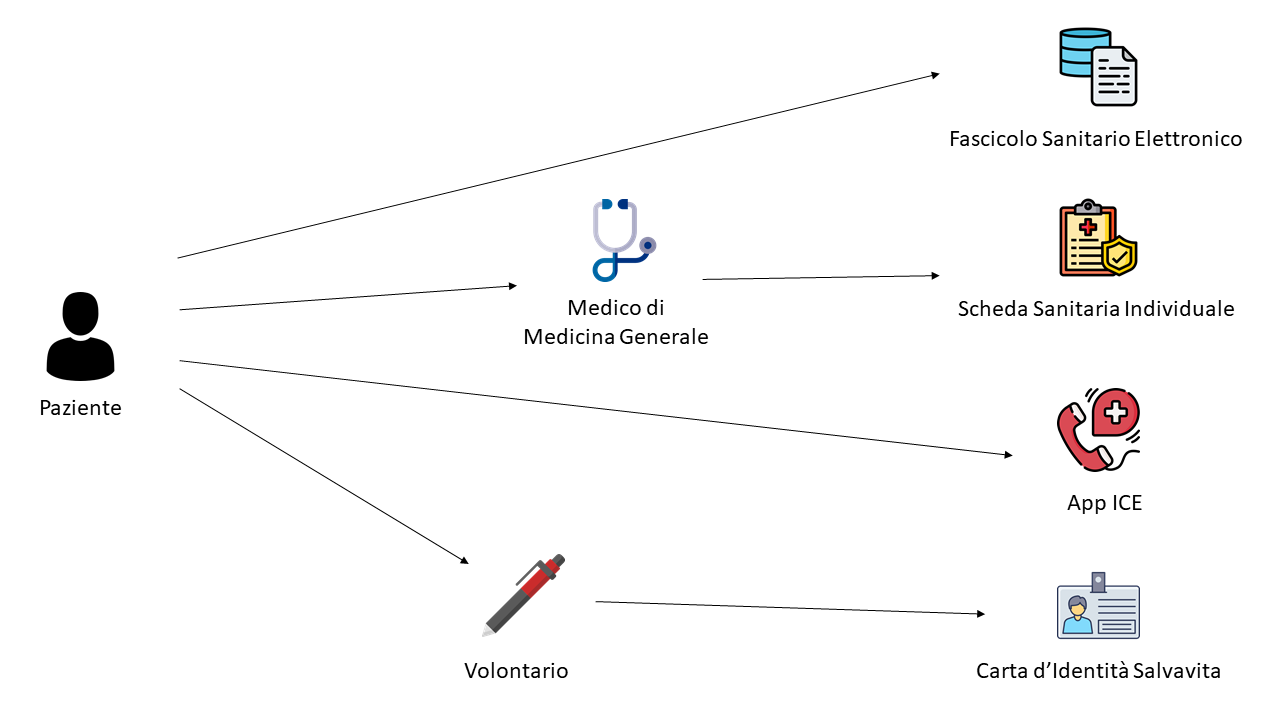
\includegraphics[scale = 0.4]{statoarte}
\caption{Stato dell'arte}
\end{figure}

\subsection{Carta d'Identità Salvavita}
Medici Volontari Italiani ha sviluppato, con l'aiuto di Fondazione IBM, Società Gisette e il Comune di Milano, un sistema in grado di digitalizzare i dati sanitari salvavita in modo che siano utilizzabili dal soccorritore in caso di necessità. Tramite l'inserimento delle informazioni del cittadino, il sistema genera la Carta d'Identità Salvavita, una tessera cartacea che presenta sulla facciata sinistra i dati anagrafici e i dati salvavita forniti dall'MMG e sulla parte destra il cosiddetto badge, ovvero un QR code riassuntivo di tali informazioni e i numeri di emergenza da contattare in caso di necessità.

\subsection{Braccialetto Salvavita}
Sviluppato parallelamente alla CIS, il braccialetto salvavita offre la possibilità di avere sempre a portata di mano il QR code la cui lettura comunica ai soccorritori le informazioni sanitarie d'emergenza definite precedentemente e segnala che la persona che lo indossa è dotata di una CIS.

\section{Obiettivo del Progetto}
Partendo dalla presenza di diverse realtà differenti che si occupano di fornire al cittadino l'obiettivo comune di salvaguardare la sua salute, questo progetto nasce con la necessità di poter crare un punto di partenza per realizzare un sistema in grado di unificare, per quanto possibile, il flusso di informazioni appena definito cercando di semplificare l'inserimento dei dati, la loro gestione e  soprattutto l'accesso e l'utilizzo da parte dei cittadini attraverso la generazione di documenti di utilità.
Il sistema realizzato salva i dati sanitari del cittadino attraverso l'applicazione web a cui hanno accesso l'MMG e il volontario, attraverso


\begin{itemize}
\item l'inserimento dei dati sanitari e salvavita del cittadino realizzato dal MMG e dal volontario;
\item l'utilizzo di queste informazioni per generare la CIS e altri documenti di utilità per il cittadino per essere sempre in grado di fornirli al soccorritore in caso di necessità.
\end{itemize}
In questo modo l'MMG è in grado di gestire e modificare i dati relativi ai suoi pazienti e i cittadini sono in grado di avere l'accesso immediato a tali dati.

\subsection{Obiettivi}
Gli obiettivi (goals) fondamentali dell'applicazione sono enunciati in seguito e sono suddivisi in:
\begin{itemize}
\item generali: riferiti all'utente generico dell'applicazione, senza alcun tipo di differenziazione tra account del volontario o account del cittadino;
\item cittadino: riferiti all'utilizzo dell'applicazione da parte del cittadino;
\item volontario: riferiti all'utilizzo dell'applicazione da parte del volontario.
\end{itemize}

\subsubsection{Generali}
\paragraph{[G1]} Permettere all'utente di eseguire il reset della password tramite l'invio via mail di un link;
\paragraph{[G2]} Mostrare una lista di numeri di emergenza che possono essere contattati in caso di necessità;
\paragraph{[G3]} Permettere all'utente di eseguire la scansione di un codice QR e mostrare i relativi dati.

\subsubsection{Cittadino}
\paragraph{[G4]} Generare partendo dai dati del cittadino il QR code, il Profilo Sanitario Sintetico, la Carta d'Identità Salvavita, il badge e il braccialetto;
\paragraph{[G5]} Permettere al cittadino di diventare utente dell'applicazione a seguito dell'inserimento dei suoi dati da parte del MMG e del volontario;
\paragraph{[G6]} Permettere all'utente di eseguire il login nel sistema attraverso l'utilizzo di valide credenziali (email e password);
\paragraph{[G7]} Mostrare all'utente il QR code che riassume le informazioni salvavita con la possibilità di aprirlo come immagine, salvarlo nel dispositivo o stamparlo in formato .pdf;
\paragraph{[G8]} Mostrare all'utente i documenti fondamentali generati dai suoi dati sanitari, quali il Profilo Sanitario Sintetico, la Carta d'Identità Salvavita, il badge e il braccialetto;
\paragraph{[G9]} Mostrare lo storico Covid dell'utente con la possibilità di aprire i documenti relativi sul web e il QR code riassuntivo degli stessi con la possibilità di aprirlo come immagine, salvarlo nel dispositivo o stamparlo in formato .pdf;
\paragraph{[G10]} Permettere all'utente di contattare l'MMG e il volontario incaricato dell'inserimento e della gestione dei dati tramite email o numero telefonico.
\paragraph{[G11]} Permettere al cittadino di selezionare i dati precedenti a quelli attuali e i relativi documenti in base alla data.

\subsubsection{Volontario}
\paragraph{[G12]} Permettere al volontario di eseguire il login nel sistema attraverso l'utilizzo di valide credenziali (email e password);
\paragraph{[G13]} Permettere al volontario di ricercare tra i cittadini a lui assegnati e selezionarli;
\paragraph{[G14]} Permettere al volontario di selezionare per il singolo cittadino i dati scelti in base alla data in cui sono stati inseriti;
\paragraph{[G15]} Permettere al volontario di stampare la Carta d'Identità Salvavita, il badge e il braccialetto di un cittadino;
\paragraph{[G16]} Permettere al volontario di stampare la Carta d'Identità Salvavita, il badge e il braccialetto a più cittadini nello stesso momento.


\chapter{Panoramica del progetto}

\section{Architettura}
L'intero sistema può essere suddiviso in 3 parti fondamentali:
\begin{itemize}
\item l'applicazione web, sviluppata da Davide Laffi, e realizzata con lo scopo di essere utilizzata dall'MMG o dal Volontario per la fase di inserimento dati sanitari e salvavita relativi al Cittadino;
\item l'applicazione mobile, sviluppata da me, e realizzata con lo scopo di essere utilizzata dal Cittadino per avere traccia delle sue informazioni sanitarie e salvavita e di conseguenza accedere ai documenti generati e dal Volontario che ha la facoltà di ricercare uno o più utenti con lo scopo di fornire servizi di utilità ai cittadini, quali la stampa dei loro documenti;
\item il lato server, realizzato utilizzando Google Firebase, e che fornisce il servizio di autenticazione per gli utenti e il servizio di database che consente il salvataggio delle informazioni relative ai cittadini.
\end{itemize}
Nelle sezioni seguenti verranno analizzate le 3 parti nel dettaglio, focalizzando l'attenzione sulle tecnologie utilizzate.\newline

\begin{figure}[H]
\centering
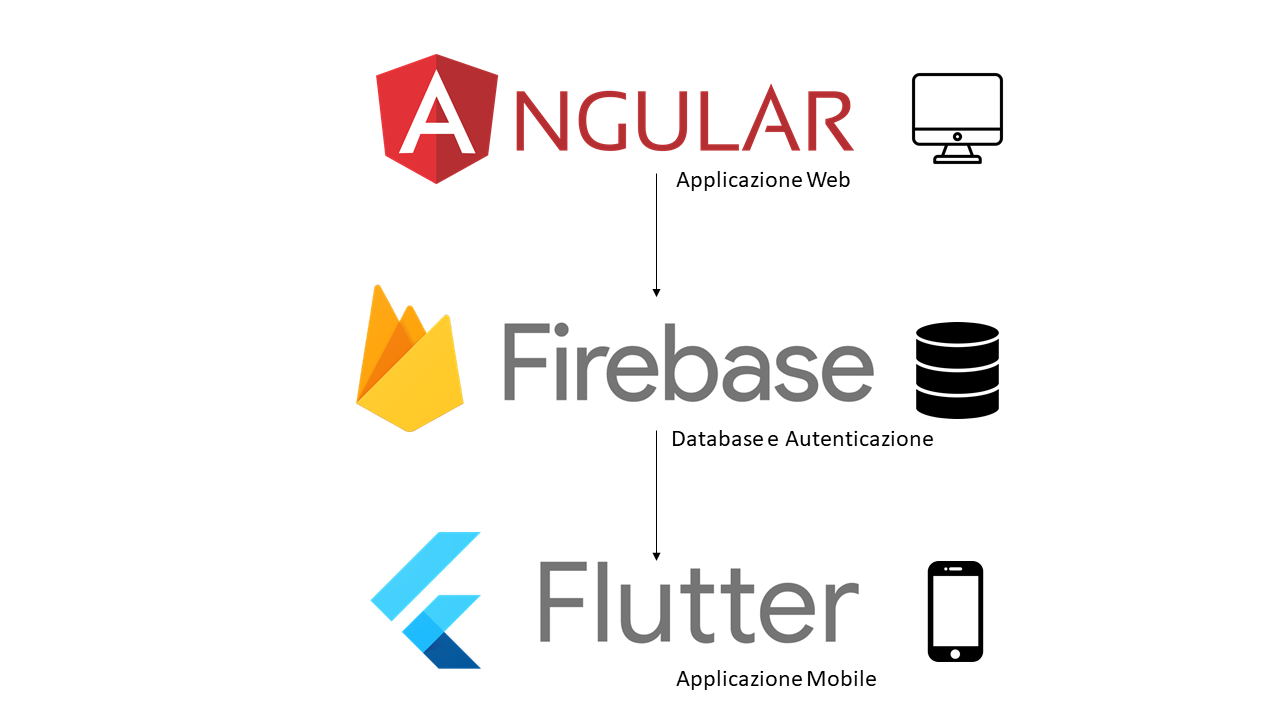
\includegraphics[scale = 0.4]{architecture}
\caption{Architettura}
\end{figure}

\section{Web Application}
L'applicazione web è stata sviluppata da Davide Laffi. Questa parte sarà descritta a seguito del lavoro di Davide.

\section{Mobile Application}
L'applicazione mobile è stata realizzata utilizzando Flutter.

\subsection{Flutter}
\textbf{Flutter} è un UI software development kit open-source creato da Google e rilasciato nel 2017 e utilizzabile per sviluppare applicazioni mobile cross-platform. Il codice di Flutter è scritto in Dart, un linguaggio di programmazione client-optimized per applicazioni su multiple piattaforme, sviluppato anch'esso da Google e utilizzato per l'implementazione di applicazioni mobile, desktop, server e web. Tra le caratteristiche principali di Flutter è bene considerare:
\begin{itemize}
\item \textbf{Cross-platform}: si basa su Dart, linguaggio unico che permette lo sviluppo su Android, iOS e sul web;
\item \textbf{Firebase}: si integra in maniera semplice e completa con Firebase;
\item \textbf{Widgets}: si compone di widgets, componenti atomiche che rappresentano elementi della UI e che possono essere uniti nella creazione di schermate pulite e complesse allo stesso tempo; 
\item \textbf{Plugins and Packages}: grazie alla vasta community di supporto esistono moltissimi packages in grado di implementare i più svariati servizi.
\end{itemize}

\section{Lato Server}
Il lato server del sistema è stato realizzato utilizzando \textbf{Google Firebase}, una piattaforma online che permette di salvare, sincronizzare e utilizzare i dati generati dalle applicazioni web e mobile. Dalla moltitudine di funzionalità offerte dal servizio, per lo sviluppo del sistema sono state utilizzate in particolare due di esse:
\begin{itemize}
\item \textbf{Autenticazione}: abilita la creazione e la gestione degli utenti per il sistema. Tra i vari metodi di sign-in disponibili è stato scelto quello classico di iscrizione e login tramite email e password. Nel servizio di autenticazione è fornita anche la possibilità del reset della password;
\item \textbf{Firestore Database}: permette la creazione di collezioni e documenti che andranno a popolare i dati che verranno utilizzati dal sistema.
\end{itemize}
Il vantaggio fondamentale nell'utilizzo di Firebase consiste nella sua perfetta integrazione con Flutter in quanto sono entrambi servizi Google.

\subsection{Autenticazione}
Poichè l'intero sistema si basa su 3 profili utente principali (MMG, volontario e cittadino), risulta necessario un servizio di autenticazione efficiente in grado servire questo scopo. In particolare l'accesso avviene tramite email e password, considerato il metodo di autenticazione più comune e scelto per:
\begin{itemize}
\item consentire ai volontari incaricati di creare gli account dei cittadini;
\item consentire alle persone meno pratiche o tecnologiche di ricordare solamente questi due parametri senza la necessità di utilizzare ulteriori fattori di autenticazione che andrebbero a complicare il processo;
\item uniformare il processo di login basandosi sul concetto che gli account social non sono posseduti da tutti, ma l'utilizzo delle mail risulta pressoché essenziale anche per i servizi più generici.
\end{itemize}
In generale i metodi di Firebase utilizzati in fase di autenticazione sono essenzialmente i seguenti:
\begin{itemize}
\item \texttt{signInWithEmailAndPassword}: consente di eseguire il login di un utente attraverso email e password nel caso in cui le credenziali fossero valide;
\item \texttt{sendPasswordResetEmail}: permette di inviare un link per il reset della password all'indirizzo email specificato.
\end{itemize}

\subsection{Firestore Database}
Cloud Firestore è un database cloud NoSQL che permette di salvare e utilizzare i dati lato client in maniera istantanea e rapida. I dati vengono sincronizzati in tempo reale e viene offerto supporto per il lavoro indipendentemente dalla latenza di rete. Le principali funzionalità offerte, reperibili nella documentazione ufficiale, sono:
\begin{itemize}
\item flessibilità: permette di organizzare i dati in collezioni e documenti;
\item interrogazione espressiva: le query possono essere utilizzate per richiedere documenti specifici o intere collezioni, attraverso l'uso di filtri e criteri di ordinamento;
\item supporto offline: i dati utilizzati dall'applicazione vengono memorizzati automaticamente nella cache in modo che il sistema possa funzionare anche in assenza di rete.
\end{itemize}
Il database del sistema è stato organizzato in 4 collezioni fondamentali:
\begin{itemize}
\item \textbf{users}: contiene un documento per ogni utente, caratterizzato dall'id utente assegnato in fase di creazione dell'account di Firebase. All'interno di ogni documento sono specificati id, codice fiscale, email e tipologia di account;
\item \textbf{patients}: contiene un documento per ogni cittadino, caratterizzato dal relativo codice fiscale. Ogni documento è collegato a sua volta ad una sottocollezione che tiene in memoria tutti i dati relativi allo storico del relativo cittadino;
\item \textbf{doctors}: contiene un documento per ogni MMG, caratterizzato dal relativo codice fiscale. Ogni documento contiene i dati anagrafici del relativo medico;
\item \textbf{volunteers}: contiene un documento per ogni volontario, caratterizzato dal relativo codice fiscale. Ogni documento contiene i dati anagrafici del relativo volontario.
\end{itemize}
Di seguito un diagramma ER che mostra più nel dettaglio le interazioni tra le varie collezioni e i campi dei singoli documenti.\newline

\textbf{IMMAGINE SCHEMATICA}

\chapter{Implementazione}
\section{Packages e Classi}
L'applicazione mobile è stata sviluppata utilizzando Flutter 2.0. Le varie classi dell'applicazione sono state suddivise in packages in base alla tipologia per incrementare la manutenibilità, la chiarezza e la separazione delle stesse.\newline

\textbf{IMMAGINE SCHEMATICA}

\subsection{Model}
\begin{figure}[H]
\centering
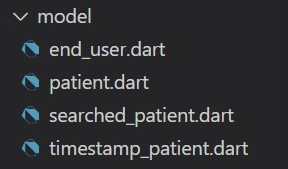
\includegraphics[scale = 1.0]{model}
\caption{The Model files}
\end{figure}
Il package Model contiene i vari oggetti utilizzati all'interno dell'applicazione che spesso si presentano con la presenza dei vari campi, del costruttore e di metodi di utilità generale per la classe. In particolare:
\begin{itemize}
\item \texttt{end\_user}: rappresenta l'utente finale dell'applicazione e permette di salvare le sue informazioni fondamentali ottenute da Firebase quali l'id, il codice fiscale, l'email e la tipologia di utente (cittadino o volontario);
\item \texttt{patient}: rappresenta il cittadino e contiene le informazioni invariabili (codice fiscale, nome e cognome) e una mappa di \texttt{TimestampPatient} organizzata per data con la funzione di storico per i dati precedenti a quelli attuali;
\item \texttt{searched\_patient}: rappresenta la classe utilizzata per gestire la ricerca dei cittadini da parte del volontario;
\item \texttt{timestamp\_patient}: contiene tutte le informazioni sanitarie e salvavita del cittadino relative ad una certa data e metodi di utilità per accedere ai dati.
\end{itemize}

\subsection{Screens}
\textbf{IMMAGINE SCHEMATICA}\newline

Il package Screens contiene le schermate principali dell'applicazione. Ogni file corrisponde ad una schermata i cui widgets sono spesso contenuti nel package Widgets. In particolare:
\begin{itemize}
\item \texttt{emergency\_numbers}: rappresenta la schermata dei Numeri Utili e si suddivide in due tabs fondamentali. La prima tab contiene i contatti (email e numero di telefono) dell'MMG e del volontario ed è costruita utilizzando le \texttt{NumbersCard}. La seconda tab contiene i numeri di emergenza da contattare in caso di necessità ed è costruita usando le \texttt{EmergencyNumberTile};
\item \texttt{homepage}: rappresenta la schermata principale dell'applicazione per quanto riguarda il cittadino. Si suddivide in 3 tab fondamentali, ovvero:
\begin{itemize}
\item QR Code: composta dal codice QR relativo alle informazioni salvavita e ai 3 \texttt{FunctionButton};
\item Informazioni: composta da 4 \texttt{FunctionCard}, ognuna relativa a un documento del cittadino;
\item Covid19: composta dal codice QR relativo allo storico Covid e ad una lista di \texttt{CovidTile}.
\end{itemize}
\item \texttt{login}: rappresenta la schermata in cui gli utenti possono effettuare l'accesso all'applicazione. È realizzata utilizzando il package \texttt{flutter\_login} che garantisce la presenza di una schermata pulita e fornita di tutte le funzionalità necessarie al suo utilizzo;
\item \texttt{qr\_code\_scanner}: rappresenta la schermata responsabile della scansione dei codici QR. Si compone di un \texttt{FunctionButton} che permette di avviare lo scanner e, in caso di scansione corretta, presenta i dati letti dal codice QR;
\item \texttt{volunteer}: rappresenta la Schermata del Volontario e si compone di una barra di ricerca realizzata attraverso il package \texttt{material\_floating\_search\_bar}. Gli utenti selezionati vengono inseriti in una lista di \texttt{VolunteerCard};
\item \texttt{wrapper}: rappresenta il widget responsabile del reindirizzamento degli utenti nella schermata corretta. Se l'utente risulta già loggato dalla sessione precedente, allora lo indirizza alla pagina relativa, altrimenti mostra la schermata di Login e attende le credenziali per reindirizzare l'utente nella Homepage (cittadino) o nella Schermata del Volontario (volontario).
\end{itemize}

\subsection{Services}
\textbf{IMMAGINE SCHEMATICA}\newline

Il package Services contiene le classi responsabili dei principali servizi utilizzati nelle varie schermate e nella logica dell'applicazione. In particolare:
\begin{itemize}
\item \texttt{auth\_service}: rappresenta la classe incaricata di gestire l'autenticazione degli utenti. Si compone dei seguenti metodi:
\begin{itemize}
\item \texttt{getCurrentUser}: restituisce l'utente Firebase corrente;
\item \texttt{login}: esegue il login dell'utente specificato attraverso email e password e restituisce un booleano rappresentante il risultato dell'operazione;
\item \texttt{resetPassword}: permette di inviare all'utente il link per il reset della password alla mail specificata.
\end{itemize}
\item \texttt{database\_service}: è la classe che si occupa della gestione del database Firebase. Ha una variabile per ogni collezione (users, patients, volunteers) e i seguenti metodi:
\begin{itemize}
\item \texttt{getUser}: restituisce il documento Firebase relativo all'utente corrente. Viene mappato nella classe \texttt{EndUser} attraverso il metodo \texttt{\_userFromFirebase};
\item \texttt{getPatient}: restituisce il documento Firebase relativo al cittadino corrente insieme ai dati sanitari e salvavita. Viene mappato nella classe \texttt{Patient} attraverso il metodo \texttt{\_patientFromFirebase};
\item \texttt{getPatientsList}: restituisce la lista dei documenti Firebase relativi a tutti i cittadini di competenza del volontario specificato.Viene mappato nella lista di \texttt{Patient} attraverso il metodo \texttt{populatePatientsData}.
\end{itemize}
\item \texttt{pdf\_handler}: è la classe che si occupa della gestione dei file in formato .pdf all'interno dell'applicazione. In particolare per ogni documento viene specificato un metodo di creazione per il file. Successivamente per ogni file è presente un metodo che si occupi di:
\begin{itemize}
\item aprire il file;
\item scaricare il file;
\item condividere il file;
\item stampare il file.
\end{itemize}
\item \texttt{qr\_code\_handler}: è la classe che si occupa della gestione dei codici QR all'interno dell'applicazione. In particolare:
\begin{itemize}
\item \texttt{generateQRCode}: genera il codice QR partendo da una stringa di dati;
\item \texttt{openQRCode}: apre il codice QR dopo averlo generato;
\item \texttt{saveQRCodeToGallery}: salva nella galleria del dispositivo il codice QR in formato immagine;
\end{itemize}
\end{itemize}

\subsection{Widgets}
\textbf{IMMAGINE SCHEMATICA}\newline

Il package Widgets contiene i widgets utilizzati frequentemente nelle altre classi dell'applicazione con l'obiettivo di ridurre al minimo la duplicazione del codice. In particolare:
\begin{itemize}
\item \texttt{appbar\_button}: rappresenta le icone cliccabili nell'appbar a cui è collegata una funzione;
\item \texttt{covid\_tile}: rappresenta le tiles presenti nello storico Covid, caratterizzate dall'evento Covid, dalla data in cui è avvenuto e dal link al documento correlato;
\item \texttt{emergency\_numbers\_tile}: rappresenta le tiles presente nella tab Emergenza dei Numeri Utili, caratterizzate da un'icona, la descrizione del contatto e il numero telefonico;
\item \texttt{form\_text\_field}:
\item \texttt{function\_button}:
\item \texttt{function\_card}:
\item \texttt{function\_icon}:
\item \texttt{numbers\_card}: rappresenta le cards presenti nella tab Contatti dei Numeri Utili, caratterizzate da un'icona, il nome, la professione (medico o volontario) e i contatti (email e numero di telefono);
\item \texttt{processing\_indicator}: rappresenta l'indicatore di caricamento presente nelle schermate dell'applicazione;
\item \texttt{radio\_tile}:
\item \texttt{volunteer\_card}: rappresenta le cards relative ai cittadini presenti nella Schermata del Volontario. Ognuna di esse si compone del nome del cittadino, il codice fiscale e i pulsanti per la stampa dei documenti relativi.
\end{itemize}

\section{External Services and Libraries}
Durante la fase di sviluppo dell'applicazione mobile è stato fatto largo utilizzo dei packages forniti dal sito \texttt{pub.dev}. Le motivazioni alla base di questa scelta sono dovute alla possibilità di sfruttare la presenza di funzionalità già esistenti per arricchire l'applicazione evitando il riutilizzo di codice e favorendo la pulizia dello stesso. Nell'elenco seguente verranno menzionati tutti i packages utilizzati con le relative funzionalità principali:
\begin{itemize}
\item \texttt{firebase\_core}: per connettere l'applicazione ai vari servizi offerti da Firebase;
\item \texttt{firebase\_auth}: per utilizzare le funzionalità di autenticazione offerte da Firebase;
\item \texttt{cloud\_firestore}: per utilizzare le funzionalità del database cloud offerto da Firebase;
\item \texttt{path\_provider}: per ottenere percorsi comuni di cartelle nei dispositivi in cui viene eseguita l'applicazione;
\item \texttt{pdf}: per generare i file .pdf utilizzati nell'applicazione e modificarli;
\item \texttt{qr\_flutter}: per generare i codici QR utilizzati per i dati salvavita e per lo storico Covid;
\item \texttt{image\_gallery\_saver}: per salvare nella galleria del dispositivo i QR code;
\item \texttt{fluttertoast}: per mostrare messaggi in rilievo a seguito di operazioni eseguite con successo;
\item \texttt{open\_file}: per aprire i file .pdf in maniera nativa nel sistema di appartenenza;
\item \texttt{downloads\_path\_provider}: per ottenere il path relativo alla cartella di Download nei dispositivi mobili;
\item \texttt{permission\_handler}: per gestire i permessi all'interno dell'applicazione;
\item \texttt{flutter\_barcode\_scanner}: per fornire la funzionalità di scansione dei codici QR;
\item \texttt{url\_launcher}: per aprire pagine internet, indirizzi email o numeri telefoni con l'applicazione di sistema correlata;
\item \texttt{humanitarian\_icons}: per avere icone aggiuntive da utilizzare nella schermata relativa ai contatti di emergenza;
\item \texttt{printing}: per abilitare le funzionalità di condivisione e stampa dei vari documenti;
\item \texttt{path}: per eseguire operazioni di manipolazione sui percorsi del sistema in uso;
\item \texttt{universal\_html}: per gestire in maniera cross-platform il package html;
\item \texttt{material\_floating\_search\_bar}: per generare una barra di ricerca consona al Material design;
\item \texttt{flutter\_login}: per generare una schermata di login pulita ed efficiente;
\item \texttt{unicorndial}: per utilizzare un floating action button con molteplici funzionalità.
\end{itemize}


\chapter{Funzionalità}
\section{Panoramica dell'Applicazione}
L'applicazione è composta da una schermata principale e da un'insieme di pagine che forniscono diverse funzionalità. In particolare l'homepage è composta da 3 tabs il cui scopo è rispettivamente di:
\begin{enumerate}
\item mostrare il QR code contentente le informazioni salvavita del cittadino con la possiblità di aprirlo come immagine, salvarlo nel dispositivo o stamparlo;
\item mostrare i documenti originali generati dai dati sanitari e dalle informazioni salvavita del cittadino con la possibilità di aprirli, salvarli nel dispositivo o stamparli;
\item mostrare uno storico relativo agli ultimi eventi relativi all'argomento Covid del cittadino (come ad esempio i tamponi o le vaccinazioni effettuati) e un QR code che riassume tutti questi eventi.
\end{enumerate}
Oltre alla schermata principale sono presenti ulteriori funzionalità che permettono all'utente di:
\begin{itemize}
\item contattare il volontario e l'MMG responsabili dell'inserimento dei dati tramite email o numero telefonico;
\item avere una lista dei numeri utili di emergenza (quali forze dell'ordine, pronto soccorso, ...), con la possibilità di contattarli in caso di necessità;
\item scannerizzare un altro QR code attraverso uno scanner integrato all'applicazione con la possibilità di mostrare i dati salvavita di un altro cittadino. Questa funzionalità è pensata per essere utilizzata dai soccorritori in caso di necessità.
\end{itemize}
Oltre alle schermate appena descritte è presente un'intera parte dell'applicazione riservata al volontario con lo scopo di abilitare la ricerca di uno o più cittadini con la facoltà di stampare per essi i documenti generati dai loro dati.

\section{Descrizione delle Funzionalità}
Nelle sezioni successive verranno analizzate nel dettaglio le funzionalità introdotte nel paragrafo precedente cercando di mettere in luce gli scopi e i modi d'utilizzo pensati.

\subsection{Registrazione}
La registrazione degli accounts avviene in due modi fondamentali in base alla tipologie di utente:
\begin{itemize}
\item volontario: la creazione dell'account del volontario (e anche quello dell'MMG) avviene per mano dell'amministratore di sistema a seguito di una richiesta. In questo modo è possibile assicurare solamente alle persone corrette il privilegio di esercitare la propria professione e avere l'accesso ai dati sensibili dei cittadini;
\item cittadino: l'account del cittadino viene creato dal volontario a seguito dell'inserimento dei dati sanitari da parte dell'MMG. In questo modo il cittadino può avere accesso all'applicazione solo a seguito dell'inserimento dei suoi dati.
\end{itemize}
Le password degli accounts sono generate in maniera randomica e inoltrate agli utenti via mail. A seguito di ciò l'utente sarà libero di modificarla secondo le proprie preferenze.

\subsection{Login}
La schermata di Login permette agli utenti di accedere al sistema fornendo credenziali valide e fornite a seguito del processo di registrazione analizzato precedentemente. Gli utenti sono in grado di modificare la propria password cliccando su "Hai dimenticato la password?" che invierà all'utente una mail contenente un link per il reset della stessa. Sia il cittadino che il volontario condividono la stessa scheramta di Login. Il sistema controlla le credenziali e reindirizza l'utente alla schermata corretta.\newline

Tramite la schermata di Login è possibile accedere, senza necessità di avere un account o di aver eseguito l'accesso, a:
\begin{itemize}
\item Numeri Utili: l'accesso senza account è stato pensato per poter utilizzare questa scheramata come una rubrica formata da tutti i numeri di emergenza accessibile in caso di necessità;
\item Scanner QR Code: l'accesso senza account è stato pensato per i soccorritori, unici veri utilizzatori di questo servizio, con l'obiettivo di velocizzare il processo di scansione il più possibile senza la necessità di possedere necessariamente un account.
\end{itemize}

\subsection{Schermata del Volontario}
Il volontario ha accesso ad una singola schermata nell'applicazione mobile in quanto la maggior parte delle sue facoltà sono correlate all'utilizzo dell'applicazione web. Il volontario, tramite un'apposita barra di ricerca, è in grado di ricercare attraverso nome o codice fiscale gli utenti di sua competenza e selezionarli. A seguito della selezione è in grado di eseguire la stampa dei documenti fondamentali (CIS, badge e braccialetto) del singolo o del gruppo di utenti selezionati. Per ogni utente, il volontario può modificare la data dei documenti scegliendo di stampare quelli richiesti.

\subsection{Homepage}
L'Homepage è la schermata principale dell'applicazione a cui ha accesso il cittadino. Questa schermata è suddivisa in 3 tabs principali che forniscono diverse funzionalità:
\begin{enumerate}
\item la prima tab mostra il QR code salvavita del cittadino contenente:
\begin{itemize}
\item Nome e cognome;
\item Data di nascita;
\item Gruppo sanguigno;
\item Primo contatto ICE;
\item Secondo contatto ICE;
\item Lista delle eventuali patologie;
\item Lista delle eventuali allergie;
\item Informazioni aggiuntive.
\end{itemize}
e permette all'utente di aprirlo come immagine, salvarlo nella galleria del dispositivo o stamparlo in formato .pdf;
\item la seconda tab mostra i documenti principali generati dai dati sanitari e salvavita inseriti dall'MMG e dal volontario incaricato:
\begin{itemize}
\item Profilo Sanitario Sintetico: contiene tutti i dati sanitari e salvavita relativi al cittadino;
\item Carta d'Identità Salvavita: mostra la CIS del cittadino contenente la foto, il QR code, i contatti ICE e le informazioni salvavita;
\item Badge: mostra la foto, il QR code e i contatti ICE;
\item Braccialetto: contiene i loghi delle società partner e il QR code.
\end{itemize}
\item la terza tab mostra gli eventi relativi alla storia Covid del cittadino, come ad esempio i tamponi effettuati o le vaccinazioni con la possibilità di aprire i documenti relativi inseriti dall'MMG o dal volontario. La schermata contiene anche un QR code riassuntivo dei vari eventi.
\end{enumerate}
Tramite l'Homepage il cittadino è in grado di accedere alle altre funzionalità dell'applicazione (Numeri Utili e Scanner QR Code) o di disconnettersi. Il cittadino può anche selezionare la data relativa ai suoi dati scegliendoli in base al periodo in cui sono stati aggiunti o modificati dall'MMG.

\subsection{Numeri Utili}
La schermata dei Numeri Utili è accessibile sia dalla schermata di Login, sia dall'Homepage e presenta due funzionalità principali:
\begin{itemize}
\item permette al cittadino loggato di contattare l'MMG e il volontario incaricato della gestione dei suoi dati tramite email o numero telefonico;
\item provvede ad una lista di numeri di emergenza che possono essere contattati dall'utente in caso di necessità:
\begin{itemize}
\item carabinieri;
\item polizia di stato;
\item vigili del fuoco;
\item guarda di finanza;
\item emergenza sanitaria.
\end{itemize}
\end{itemize}

\subsection{Scanner QR Code}
La schermata dello Scanner è accessibile sia dalla schermata di Login, sia dall'Homepage. Questa funzionalità è stata pensata per essere utilizzata dai soccorritori che, senza dover necessariamente fare l'accesso all'applicazione, possono utilizzare lo scanner QR per avere accesso immediato alle informazioni salvavita dei cittadini in difficoltà. L'applicazione infatti, a seguito della scansione, mostra i dati del cittadino in forma leggibile ed organizzata.

\chapter{Interfaccia Utente e Casi d'Uso}
\section{UI Design}
Il design dell'interfaccia utente è basato principalmente sulle linee guida del Material design, cercando di focalizzarsi simultaneamente su:
\begin{itemize}
\item semplicità d'uso: garantita dalle schermate pulite e prive di troppi elementi a schermo, cercando di rendere chiaro all'utente lo scopo di ogni singola componente;
\item efficienza: garantita dalla presenza di singole operazioni atomiche che non bloccano eccessivamente l'utilizzo dell'applicazione all'utente.
\end{itemize}
Nei prossimi paragrafi verranno analizzate in dettaglio le scelte stilistiche e progettuali volte a soddisfare i requisiti appena definiti, focalizzandosi sulle motivazioni di tali scelte e mostrando le schermate fondamentali dell'applicazione.

\subsection{Logo}
\subsection{Schermate Principali}
\subsection{Layout Web}

\section{Use Cases}
Nelle sezioni successive verrano analizzate i casi d'uso più frequenti, avendo cura di specificare:
\begin{itemize}
\item Scenario: il titolo riassuntivo del caso d'uso analizzato;
\item Condizione d'ingresso: requisiti minimi per l'esecuzione del caso d'uso;
\item Flusso degli eventi: azioni o avvenimenti che caratterizzano il caso d'uso;
\item Condizione d'uscita: evento finale che termina il flusso degli eventi;
\item Eccezioni: possibili avvenimenti che causano l'interruzione o privano l'esecuzione degli eventi.
\end{itemize}


\subsection{Login}
\begin{table}[H]
\centering
\begin{tabular}{|p{4cm}|p{10cm}|}
\hline
Scenario & Login utente \\
\hline
Condizione d'ingresso & L'utente ha scaricato l'applicazione o ha eseguito l'accesso attraverso il web browser \newline
L'utente ha già un account creato dal volontario incaricato \\
\hline
Flusso degli eventi & 
\begin{enumerate}
\item L'utente inserisce la sua email nel campo "Email" della schermata
\item L'utente inserisce la sua password nel campo "Password" della schermata
\item L'utente clicca sul bottone di "Login"
\end{enumerate}\\
\hline
Condizione d'uscita & L'applicazione reindirizza l'utente nella schermata corretta, in base alla tipologia di account (cittadino o volontario)\\
\hline
Eccezioni & 
\begin{itemize}
\item L'utente non ha inserito credenziali valide
\item L'utente non ha inserito le credenziali in tutti i campi obbligatori
\item Il sistema non è in grado di completare la richiesta a causa di un errore interno
\end{itemize} \\
\hline
\end{tabular}
\end{table}

\begin{table}[H]
\centering
\begin{tabular}{|p{4cm}|p{10cm}|}
\hline
Scenario & Reset della password \\
\hline
Condizione d'ingresso & L'utente ha scaricato l'applicazione o ha eseguito l'accesso attraverso il web browser \newline
L'utente ha già un account creato dal volontario incaricato \\
\hline
Flusso degli eventi & 
\begin{enumerate}
\item L'utente clicca sulla scritta "Password dimenticata?"
\item L'applicazione mostra il form per il reset della password
\item L'utente inserisce la sua email nel campo "Email" della schermata
\item L'utente clicca sul bottone di "Reset"
\end{enumerate}\\
\hline
Condizione d'uscita & L'applicazione mostra un messaggio di successo\\
\hline
Eccezioni & 
\begin{itemize}
\item L'utente non ha inserito credenziali valide
\item L'utente non ha inserito l'email nel campo relativo
\item Il sistema non è in grado di completare la richiesta a causa di un errore interno
\end{itemize} \\
\hline
\end{tabular}
\end{table}

\subsection{Logout}
\begin{table}[H]
\centering
\begin{tabular}{|p{4cm}|p{10cm}|}
\hline
Scenario & Cambio schermata \\
\hline
Condizione d'ingresso & L'utente è nella schermata di Homepage o nella Schermata del Volontario\\
\hline
Flusso degli eventi & 
\begin{enumerate}
\item L'utente clicca sull'icona relativa alla logout in alto a sinistra
\end{enumerate}\\
\hline
Condizione d'uscita & L'applicazione esegue il logout dell'utente e lo reindirizza alla schermata di Login
\\
\hline
Eccezioni & 
\begin{itemize}
\item Il sistema non è in grado di completare la richiesta a causa di un errore interno
\end{itemize} \\
\hline
\end{tabular}
\end{table}

\subsection{Homepage}
\begin{table}[H]
\centering
\begin{tabular}{|p{4cm}|p{10cm}|}
\hline
Scenario & Cambio schermata \\
\hline
Condizione d'ingresso & L'utente è nella schermata di Homepage\\
\hline
Flusso degli eventi & 
\begin{enumerate}
\item L'utente clicca sull'icona relativa alla schermata scelta in alto a destra (Numeri Utili o Scanner QR)
\end{enumerate}\\
\hline
Condizione d'uscita & L'applicazione reindirizza l'utente nella schermata scelta
\\
\hline
Eccezioni & 
\begin{itemize}
\item Il sistema non è in grado di completare la richiesta a causa di un errore interno
\end{itemize} \\
\hline
\end{tabular}
\end{table}

\begin{table}[H]
\centering
\begin{tabular}{|p{4cm}|p{10cm}|}
\hline
Scenario & Scelta documenti \\
\hline
Condizione d'ingresso & L'utente è nella schermata di Homepage\\
\hline
Flusso degli eventi & 
\begin{enumerate}
\item L'utente clicca sull'icona relativa al menu in alto a destra della schermata
\item L'applicazione mostra le date relative allo storico dell'utente
\item L'utente clicca sulla data scelta
\end{enumerate}\\
\hline
Condizione d'uscita & L'applicazione aggiorna i dati del cittadino mostrando quelli relativi alla data scelta
\\
\hline
Eccezioni & 
\begin{itemize}
\item Il cittadino non dispone di altre date tra cui scegliere oltre a quella attuale
\item Il sistema non è in grado di completare la richiesta a causa di un errore interno
\end{itemize} \\
\hline
\end{tabular}
\end{table}

\begin{table}[H]
\centering
\begin{tabular}{|p{4cm}|p{10cm}|}
\hline
Scenario & Codice QR \\
\hline
Condizione d'ingresso & L'utente è nella schermata di Homepage, nella tab Codice QR\\
\hline
Flusso degli eventi & 
\begin{enumerate}
\item L'utente clicca sul bottone:
\begin{itemize}
\item "Apri"
\item "Salva"
\item "Stampa"
\end{itemize}
\item L'applicazione esegue l'azione richiesta
\end{enumerate}\\
\hline
Condizione d'uscita & L'applicazione:
\begin{itemize}
\item apre il codice QR come immagine
\item salva nel dispositivo il codice QR come immagine
\item apre la schermata di stampa per il codice QR in formato .pdf
\end{itemize}\\
\hline
Eccezioni & 
\begin{itemize}
\item Il sistema non è in grado di completare la richiesta a causa di un errore interno
\end{itemize} \\
\hline
\end{tabular}
\end{table}

\begin{table}[H]
\centering
\begin{tabular}{|p{4cm}|p{10cm}|}
\hline
Scenario & Informazioni \\
\hline
Condizione d'ingresso & L'utente è nella schermata di Homepage, nella tab Informazioni\\
\hline
Flusso degli eventi & 
\begin{enumerate}
\item L'utente sceglie il documento di interesse:
\begin{itemize}
\item Dati
\item Badge
\item CIS
\item Braccialetto
\end{itemize}
\item L'utente clicca sull'icona relativa a:
\begin{itemize}
\item "Apri"
\item "Salva"
\item "Stampa"
\end{itemize}
\item L'applicazione genera il documento ed esegue l'azione richiesta
\end{enumerate}\\
\hline
Condizione d'uscita & L'applicazione:
\begin{itemize}
\item apre il documento in formato .pdf
\item salva nel dispositivo il documento in formato .pdf
\item apre la schermata di stampa per documento in formato .pdf
\end{itemize}\\
\hline
Eccezioni & 
\begin{itemize}
\item Il sistema non è in grado di completare la richiesta a causa di un errore interno
\end{itemize} \\
\hline
\end{tabular}
\end{table}

\begin{table}[H]
\centering
\begin{tabular}{|p{4cm}|p{10cm}|}
\hline
Scenario & Covid19 - QR code\\
\hline
Condizione d'ingresso & L'utente è nella schermata di Homepage, nella tab Covid19\\
\hline
Flusso degli eventi & 
\begin{enumerate}
\item L'utente clicca sul bottone:
\begin{itemize}
\item "Apri"
\item "Salva"
\item "Stampa"
\end{itemize}
\item L'applicazione esegue l'azione richiesta
\end{enumerate}\\
\hline
Condizione d'uscita & L'applicazione:
\begin{itemize}
\item apre il codice QR come immagine
\item salva nel dispositivo il codice QR come immagine
\item apre la schermata di stampa per il codice QR in formato .pdf
\end{itemize}\\
\hline
Eccezioni & 
\begin{itemize}
\item Il sistema non è in grado di completare la richiesta a causa di un errore interno
\end{itemize} \\
\hline
\end{tabular}
\end{table}

\begin{table}[H]
\centering
\begin{tabular}{|p{4cm}|p{10cm}|}
\hline
Scenario & Covid19 - Storico\\
\hline
Condizione d'ingresso & L'utente è nella schermata di Homepage, nella tab Covid19\\
\hline
Flusso degli eventi & 
\begin{enumerate}
\item L'utente sceglie dalla lista l'evento di interesse
\item L'utente clicca sul bottone "Apri"
\item L'applicazione esegue l'azione richiesta
\end{enumerate}\\
\hline
Condizione d'uscita & L'applicazione apre il documento richiesto nella pagina web di provenienza\\
\hline
Eccezioni & 
\begin{itemize}
\item L'utente non ha alcun dato nello storico Covid
\item Il sistema non è in grado di completare la richiesta a causa di un errore interno
\end{itemize} \\
\hline
\end{tabular}
\end{table}

\subsection{Schermata del Volontario}
\begin{table}[H]
\centering
\begin{tabular}{|p{4cm}|p{10cm}|}
\hline
Scenario & Ricerca cittadino \\
\hline
Condizione d'ingresso & Il volontario ha scaricato l'applicazione o ha eseguito l'accesso attraverso il web browser \newline
Il volontario ha già un account \\
\hline
Flusso degli eventi & 
\begin{enumerate}
\item Il volontario inserisce il nome (o il codice fiscale) del cittadino di sua competenza nella barra di ricerca che presenta la scritta "Cerca..."
\item L'applicazione mostra i cittadini che soddisfano la ricerca del volontario
\item Il volontario seleziona il cittadino (o i cittadini) desiderato cliccando il pulsante "Aggiungi"
\end{enumerate}\\
\hline
Condizione d'uscita & L'applicazione aggiunge alla lista il cittadino selezionato e lo mostra nella schermata\\
\hline
Eccezioni & 
\begin{itemize}
\item Il volontario ha inserito un nome (o un codice fiscale) inesistente
\item Il cittadino non fa parte delle competenze del volontario
\item Il sistema non è in grado di completare la richiesta a causa di un errore interno
\end{itemize} \\
\hline
\end{tabular}
\end{table}

\begin{table}[H]
\centering
\begin{tabular}{|p{4cm}|p{10cm}|}
\hline
Scenario & Rimozione cittadino \\
\hline
Condizione d'ingresso & Il volontario ha scaricato l'applicazione o ha eseguito l'accesso attraverso il web browser \newline
Il volontario ha già un account\newline
Il volontario ha selezionato un cittadino attraverso la barra di ricerca\\
\hline
Flusso degli eventi & 
\begin{enumerate}
\item Il volontario seleziona il cittadino di interesse tra quelli presenti nella lista
\item Il volontario clicca sull'icona ad X nella scheda relativa al cittadino
\end{enumerate}\\
\hline
Condizione d'uscita & L'applicazione rimuove dalla lista il cittadino selezionato\\
\hline
Eccezioni & 
\begin{itemize}
\item Il sistema non è in grado di completare la richiesta a causa di un errore interno
\end{itemize} \\
\hline
\end{tabular}
\end{table}

\begin{table}[H]
\centering
\begin{tabular}{|p{4cm}|p{10cm}|}
\hline
Scenario & Scelta documenti cittadino \\
\hline
Condizione d'ingresso & Il volontario ha scaricato l'applicazione o ha eseguito l'accesso attraverso il web browser \newline
Il volontario ha già un account\newline
Il volontario ha selezionato un cittadino attraverso la barra di ricerca \\
\hline
Flusso degli eventi & 
\begin{enumerate}
\item Il volontario seleziona il cittadino di interesse tra quelli presenti nella lista
\item Il volontario clicca sull'icona rappresentante il menu nella scheda relativa al cittadino
\item Il volontario clicca sulla data di interesse
\end{enumerate}\\
\hline
Condizione d'uscita & L'applicazione aggiorna i dati del cittadino mostrando quelli relativi alla data scelta\\
\hline
Eccezioni & 
\begin{itemize}
\item Il cittadino selezionato non dispone di altre date tra cui scegliere oltre a quella attuale
\item Il sistema non è in grado di completare la richiesta a causa di un errore interno
\end{itemize} \\
\hline
\end{tabular}
\end{table}

\begin{table}[H]
\centering
\begin{tabular}{|p{4cm}|p{10cm}|}
\hline
Scenario & Stampa singola \\
\hline
Condizione d'ingresso & Il volontario ha scaricato l'applicazione o ha eseguito l'accesso attraverso il web browser \newline
Il volontario ha già un account\newline
Il volontario ha selezionato un cittadino attraverso la barra di ricerca \\
\hline
Flusso degli eventi & 
\begin{enumerate}
\item Il volontario seleziona il cittadino di interesse tra quelli presenti nella lista
\item Il volontario seleziona il documento di interesse tra Badge, CIS e Braccialetto
\item Il volontario clicca sul pulsante "Stampa"
\end{enumerate}\\
\hline
Condizione d'uscita & L'applicazione mostra la schermata di stampa del documento selezionato in formato .pdf\\
\hline
Eccezioni & 
\begin{itemize}
\item Il sistema non è in grado di completare la richiesta a causa di un errore interno
\end{itemize} \\
\hline
\end{tabular}
\end{table}

\begin{table}[H]
\centering
\begin{tabular}{|p{4cm}|p{10cm}|}
\hline
Scenario & Stampa multipla \\
\hline
Condizione d'ingresso & Il volontario ha scaricato l'applicazione o ha eseguito l'accesso attraverso il web browser \newline
Il volontario ha già un account\newline
Il volontario ha selezionato più cittadini attraverso la barra di ricerca \\
\hline
Flusso degli eventi & 
\begin{enumerate}
\item Il volontario clicca sul pulsante in basso a destra dello schermo che presenta l'icona di stampa
\item Il volontario seleziona il documento di interesse cliccando sull'icon corrispondente
\end{enumerate}\\
\hline
Condizione d'uscita & L'applicazione mostra la schermata di stampa dei documenti selezionati in formato .pdf\\
\hline
Eccezioni & 
\begin{itemize}
\item Il sistema non è in grado di completare la richiesta a causa di un errore interno
\end{itemize} \\
\hline
\end{tabular}
\end{table}

\subsection{Numeri Utili}
\begin{table}[H]
\centering
\begin{tabular}{|p{4cm}|p{10cm}|}
\hline
Scenario & Contatti \\
\hline
Condizione d'ingresso & L'utente ha scaricato l'applicazione o ha eseguito l'accesso attraverso il web browser\newline
L'utente ha già un account creato dal volontario incaricato\newline
L'utente è nella schermata Numeri Utili, nella tab Contatti\\
\hline
Flusso degli eventi & 
\begin{enumerate}
\item L'utente sceglie il contatto desiderato tra MMG e volontario
\item L'utente clicca sulla forma di comunicazione desiderata (numero telefonico o email)
\end{enumerate}\\
\hline
Condizione d'uscita & L'applicazione apre l'applicazione del dispositivo in grado di gestire la richiesta\\
\hline
Eccezioni & 
\begin{itemize}
\item Il sistema non è in grado di completare la richiesta a causa di un errore interno
\end{itemize} \\
\hline
\end{tabular}
\end{table}

\begin{table}[H]
\centering
\begin{tabular}{|p{4cm}|p{10cm}|}
\hline
Scenario & Contatti \\
\hline
Condizione d'ingresso & L'utente ha scaricato l'applicazione o ha eseguito l'accesso attraverso il web browser\newline
L'utente è nella schermata Numeri Utili, nella tab Emergenza\\
\hline
Flusso degli eventi & 
\begin{enumerate}
\item L'utente sceglie il contatto desiderato tra Carabinieri, Polizia di Stato, Vigili del Fuoco, Guardia di Finanza e Emergenza Sanitaria
\item L'utente clicca sul contatto desiderato
\end{enumerate}\\
\hline
Condizione d'uscita & L'applicazione apre l'applicazione del dispositivo in grado di gestire la richiesta\\
\hline
Eccezioni & 
\begin{itemize}
\item Il sistema non è in grado di completare la richiesta a causa di un errore interno
\end{itemize} \\
\hline
\end{tabular}
\end{table}

\subsection{QR Code Scanner}
\begin{table}[H]
\centering
\begin{tabular}{|p{4cm}|p{10cm}|}
\hline
Scenario & Scansione QR \\
\hline
Condizione d'ingresso & L'utente ha scaricato l'applicazione\newline
L'utente è nella schermata QR Code Scanner\\
\hline
Flusso degli eventi & 
\begin{enumerate}
\item L'utente clicca sul pulsante "Scan"
\item L'applicazione attiva la camera del dispositivo in attesa della scansione
\item L'utente esegue la scansione di un codice QR
\end{enumerate}\\
\hline
Condizione d'uscita & L'applicazione mostra i dati relativi al codice QR scansionato\\
\hline
Eccezioni & 
\begin{itemize}
\item L'utente cerca di eseguire la scansione di un codice QR che non soddisfa i requisiti dell'applicazione
\item Il sistema non è in grado di completare la richiesta a causa di un errore interno
\end{itemize} \\
\hline
\end{tabular}
\end{table}

\section{User-Flow Diagram}
Il grafico seguente mostra nel dettaglio tutte le possibili interazioni tra le schermate dell'applicazione attraverso un user flow diagram.


\chapter{Conclusione e Sviluppi Futuri}
Il sistema realizzato riesce a concentrare in un unico flusso la fase di inserimento dei dati sanitari e salvavita del cittadino e il loro utilizzo per garantire servizi di utilità e salvaguardia per gli utenti finali. Sebbene realizzato con dati fittizi e senza la presunzione di andare a sostituire quanto già in uso, si propone come un'idea con cui poter sviluppare, in futuro, un sistema complessivo in grado di gestire interamente questo tipo di informazioni e dati per poterne semplificare l'accesso e l'uso.\newline

Come già analizzato brevemente all'inizio di questa trattazione, lo stato dell'arte presenta numerosi sistemi proprietari che non si interfacciano e rendono spesso complicata l'interazione o l'accesso ai propri cittadini. Realizzato quanto fatto, poniamo le basi per un sistema in grado di interfacciarsi con le differenti realtà presenti.\newline

L'inserimento della schermata relativa al Covid19 risulta sicuramente volto all'utilità che potrebbe conseguirne soprattutto in questo periodo storico in cui avere a portata di mano i documenti relativi a tamponi e vaccinazioni può rappresentare un vantaggio notevole a livello di utilità, ma più che altro mostra come il sistema realizzato sia in grado di integrare, all'occorrenza, nuove funzionalità che possano aiutare i cittadini nella loro vita sanitaria cercando di inglobare in un unico accesso quanti più dati e servizi utili per gli stessi.\newline

Partendo da quanto fatto ci auguriamo che il lavoro realizzato possa fornire spunti interessanti per lo sviluppo futuro di un sistema completo e coerente dotato di tutte le caratteristiche necessarie per aiutare il cittadino nella gestione e nell'accesso a dati fondamentali come quelli sanitari.

\chapter{Bibliografia}
Di seguito le fonti utilizzate per la stesura del documento e la realizzazione del progetto:
\begin{itemize}
\item \href{https://www.medicivolontaritaliani.org/}{Medici Volontari Italiani};
\item \href{https://www.comune.milano.it/aree-tematiche/servizi-sociali/raccolta-dati-personali-per-interventi-di-emergenza}{Comune di Milano};
\end{itemize}

\end{document}